\renewcommand{\theequation}{\theenumi}
\begin{enumerate}[label=\arabic*.,ref=\thesubsubsection.\theenumi]
\numberwithin{equation}{enumi}
%
\item From the given information,
\begin{align}
\norm{\vec{x}-\myvec{2\\-5}}^2 = \norm{\vec{x}-\myvec{-2\\9}}^2 
\end{align}
$\norm{\vec{x}}^2+\norm{\myvec{2\\-5}}^2-2\myvec{2 & -5}\vec{x} = \norm{\vec{x}}^2+\norm{\myvec{-2\\9}}^2-2\myvec{-2 & 9}\vec{x}$ \\
which can be simplified to obtain
\begin{align}
\myvec{8 & -28}\vec{x} = -56
\end{align}
Choose $\vec{x} = \myvec{x\\0}$ as the point lies on the x-axis
\begin{align}
\myvec{8 & -28}\myvec{x\\0} = -56
\\
\implies x = -7
\end{align}

The point is $\myvec{-7\\0}$  

The Lines in Fig.\ref{fig:line_1} is generated using the following python code 
\begin{lstlisting}
codes/line/point_vector/point_vector.py
\end{lstlisting}

\begin{figure}[!ht]
\centering
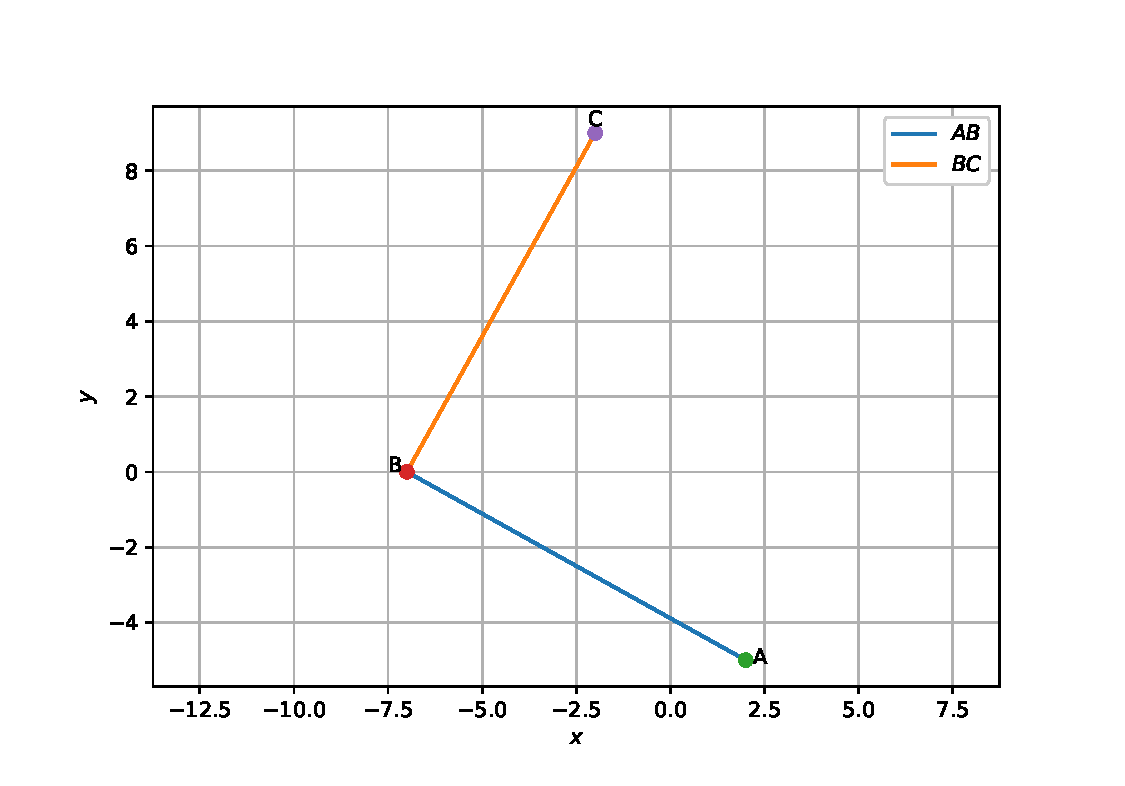
\includegraphics[width=\columnwidth]{./codes/line/point_vector/point_vector.eps}
\caption{Lines generated using python}
\label{fig:line_1}
\end{figure}

\end{enumerate}

